\documentclass{sigchi}

%Conference
\conferenceinfo{Ortega '19,}{December  18, 2019, Fort Collins, CO, USA}

\pagenumbering{arabic}

% Load basic packages
\usepackage{balance}       % to better equalize the last page
\usepackage{graphics}      % for EPS, load graphicx instead 
\usepackage[T1]{fontenc}   % for umlauts and other diaeresis
\usepackage{txfonts}
\usepackage{mathptmx}
\usepackage[pdflang={en-US},pdftex]{hyperref}
\usepackage{color}
\usepackage{booktabs}
\usepackage{textcomp}

% Some optional stuff you might like/need.
\usepackage{microtype}        % Improved Tracking and Kerning
% \usepackage[all]{hypcap}    % Fixes bug in hyperref caption linking
\usepackage{ccicons}          % Cite your images correctly!
% \usepackage[utf8]{inputenc} % for a UTF8 editor only

% If you want to use todo notes, marginpars etc. during creation of
% your draft document, you have to enable the "chi_draft" option for
% the document class. To do this, change the very first line to:
% "\documentclass[chi_draft]{sigchi}". You can then place todo notes
% by using the "\todo{...}"  command. Make sure to disable the draft
% option again before submitting your final document.
\usepackage{todonotes}

% Paper metadata (use plain text, for PDF inclusion and later
% re-using, if desired).  Use \emtpyauthor when submitting for review
% so you remain anonymous.
\def\plaintitle{SIGCHI Conference Proceedings Format}
\def\plainauthor{First Author, Second Author, Third Author,
  Fourth Author, Fifth Author, Sixth Author}
\def\emptyauthor{}
\def\plainkeywords{Human-Computer Interaction; 3D Dynamics; Unmanned Aerial Vehicle; Bridges; Structural Health Monitoring.}
\def\plaingeneralterms{Documentation, Standardization}

% llt: Define a global style for URLs, rather that the default one
\makeatletter
\def\url@leostyle{%
  \@ifundefined{selectfont}{
    \def\UrlFont{\sf}
  }{
    \def\UrlFont{\small\bf\ttfamily}
  }}
\makeatother
\urlstyle{leo}

% To make various LaTeX processors do the right thing with page size.
\def\pprw{8.5in}
\def\pprh{11in}
\special{papersize=\pprw,\pprh}
\setlength{\paperwidth}{\pprw}
\setlength{\paperheight}{\pprh}
\setlength{\pdfpagewidth}{\pprw}
\setlength{\pdfpageheight}{\pprh}

% Make sure hyperref comes last of your loaded packages, to give it a
% fighting chance of not being over-written, since its job is to
% redefine many LaTeX commands.
\definecolor{linkColor}{RGB}{6,125,233}
\hypersetup{%
  pdftitle={\plaintitle},
% Use \plainauthor for final version.
%  pdfauthor={\plainauthor},
  pdfauthor={\emptyauthor},
  pdfkeywords={\plainkeywords},
  pdfdisplaydoctitle=true, % For Accessibility
  bookmarksnumbered,
  pdfstartview={FitH},
  colorlinks,
  citecolor=black,
  filecolor=black,
  linkcolor=black,
  urlcolor=linkColor,
  breaklinks=true,
  hypertexnames=false
}

% create a shortcut to typeset table headings
% \newcommand\tabhead[1]{\small\textbf{#1}}

% End of preamble. Here it comes the document.
\begin{document}

\title{\plaintitle}

\numberofauthors{1}
\author{%
  \alignauthor{Brandon J. Perry\\
    \affaddr{Colorado State University}\\
    \affaddr{Fort Collins, CO, USA}\\
    \email{bjperry@colostate.edu}}\\
}

\maketitle

\begin{abstract}
  Fully understanding the bridge performance under traffic loadings is critical for improving bridge design, condition assessment, and load rating. Modern structural health monitoring (SHM) has enabled measurements of the traffic loads and dynamic bridge response to help enhance the knowledge on the mechanism of vehicle-bridge interactions; however, challenges still exist for accurately measuring the exact moving traffic loads and the corresponding traffic induced response. Recently, with the tremendous advancements in unmanned aerial vehicles (UAVs) technology (including better camera performance and longer flight times), UAVs can offer unique advantages to hover at specified heights and key locations and access difficult to reach areas and critical angles while providing relatively stable and high-quality imagery. By leveraging the recent advantages in UAV technologies, image computation, and camera vision-based SHM, this study proposes a UAV-based SHM system to track vehicular loading and measure the displacement of the bridge simultaneously. In the system, a UAV will hover adjacent to a bridge measuring the structure`s response. Then, an object identification algorithm will be developed to identify and track moving trucks. Digital image correlation technique will be employed to quantify the three-dimensional dynamic displacement of the bridge. Additionally, to facilitate adoption of the proposed system, a user-friendly interface will be developed to easily identify displacements of key 3D points.This proposed system will provide valuable data for accurate modeling and assessment of bridge performance under traffic loads.
\end{abstract}

% Author Keywords
\keywords{\plainkeywords}

\section{Project Overview, Timeline, and Deliverables}

The project will begin with first performing static testing of the equipment. \cite{Nguyen2017} has shown tremendous success using the same instrumentation within a static system with known, controlled variables. Replicating these results will be the first task. Next, the visualization of the information will be studied. The output from the system needs to provide a user-friendly interface to access and interpret the information. Lastly, if time permits, the tests will be performed using the same setup, but with the sensors installed on a UAV. The final deliverable will be the algorithm to measure 3D displacement of a structure using either the static, or dynamic setup of the equipment. Additionally, a user-friendly interface for a user to view and analyze the results will be built. This interface will include a 3D point cloud of the object as the object moves and some graphs and tables of the movement and results in real-time (if feasible).

\section{Proposed Technology Usage}
The proposed technology includes:

\begin{quote}
    1. Two Intel RealSense D435 Depth Cameras
\end{quote} 

\begin{quote}
    \begin{quote}
       This camera uses an infrared projector to create a virtual speckle pattern on a subject and two infrared receives which can measure the movement of the virtual speckle pattern. Shown in Figure \ref{fig:1} 
    \end{quote}
\end{quote} 

\begin{figure}
\centering
    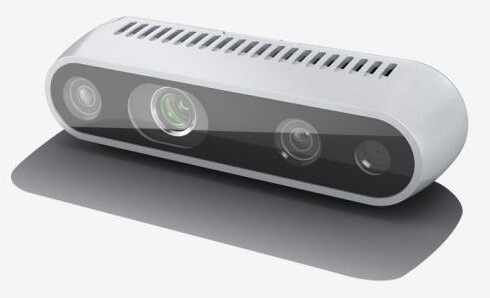
\includegraphics[width=0.9\columnwidth]{Figures/Intel_RealSense_D435.jpg}
    \caption{Intel RealSense D435 Depth Camera}
    \label{fig:1}
\end{figure}

\begin{quote}
    2. Microsoft Surface Computer
\end{quote} 

\begin{quote}
    \begin{quote}
       This computer will provide a user-friendly interaction to easily visualize and interact with the output from the designed system
    \end{quote}
\end{quote}

\begin{quote}
    2. DJI Matrice 600 Pro
\end{quote} 

\begin{quote}
    \begin{quote}
       This UAV is a large and robust system capable of carrying the needed instruments while maintaining 30-\textit{minutes} of flight time. If the preliminary, static test perform well, the UAV will be incorporated into the project. The UAV can be seen in Figure \ref{fig:2}.
    \end{quote}
\end{quote}

\begin{figure}
\centering
    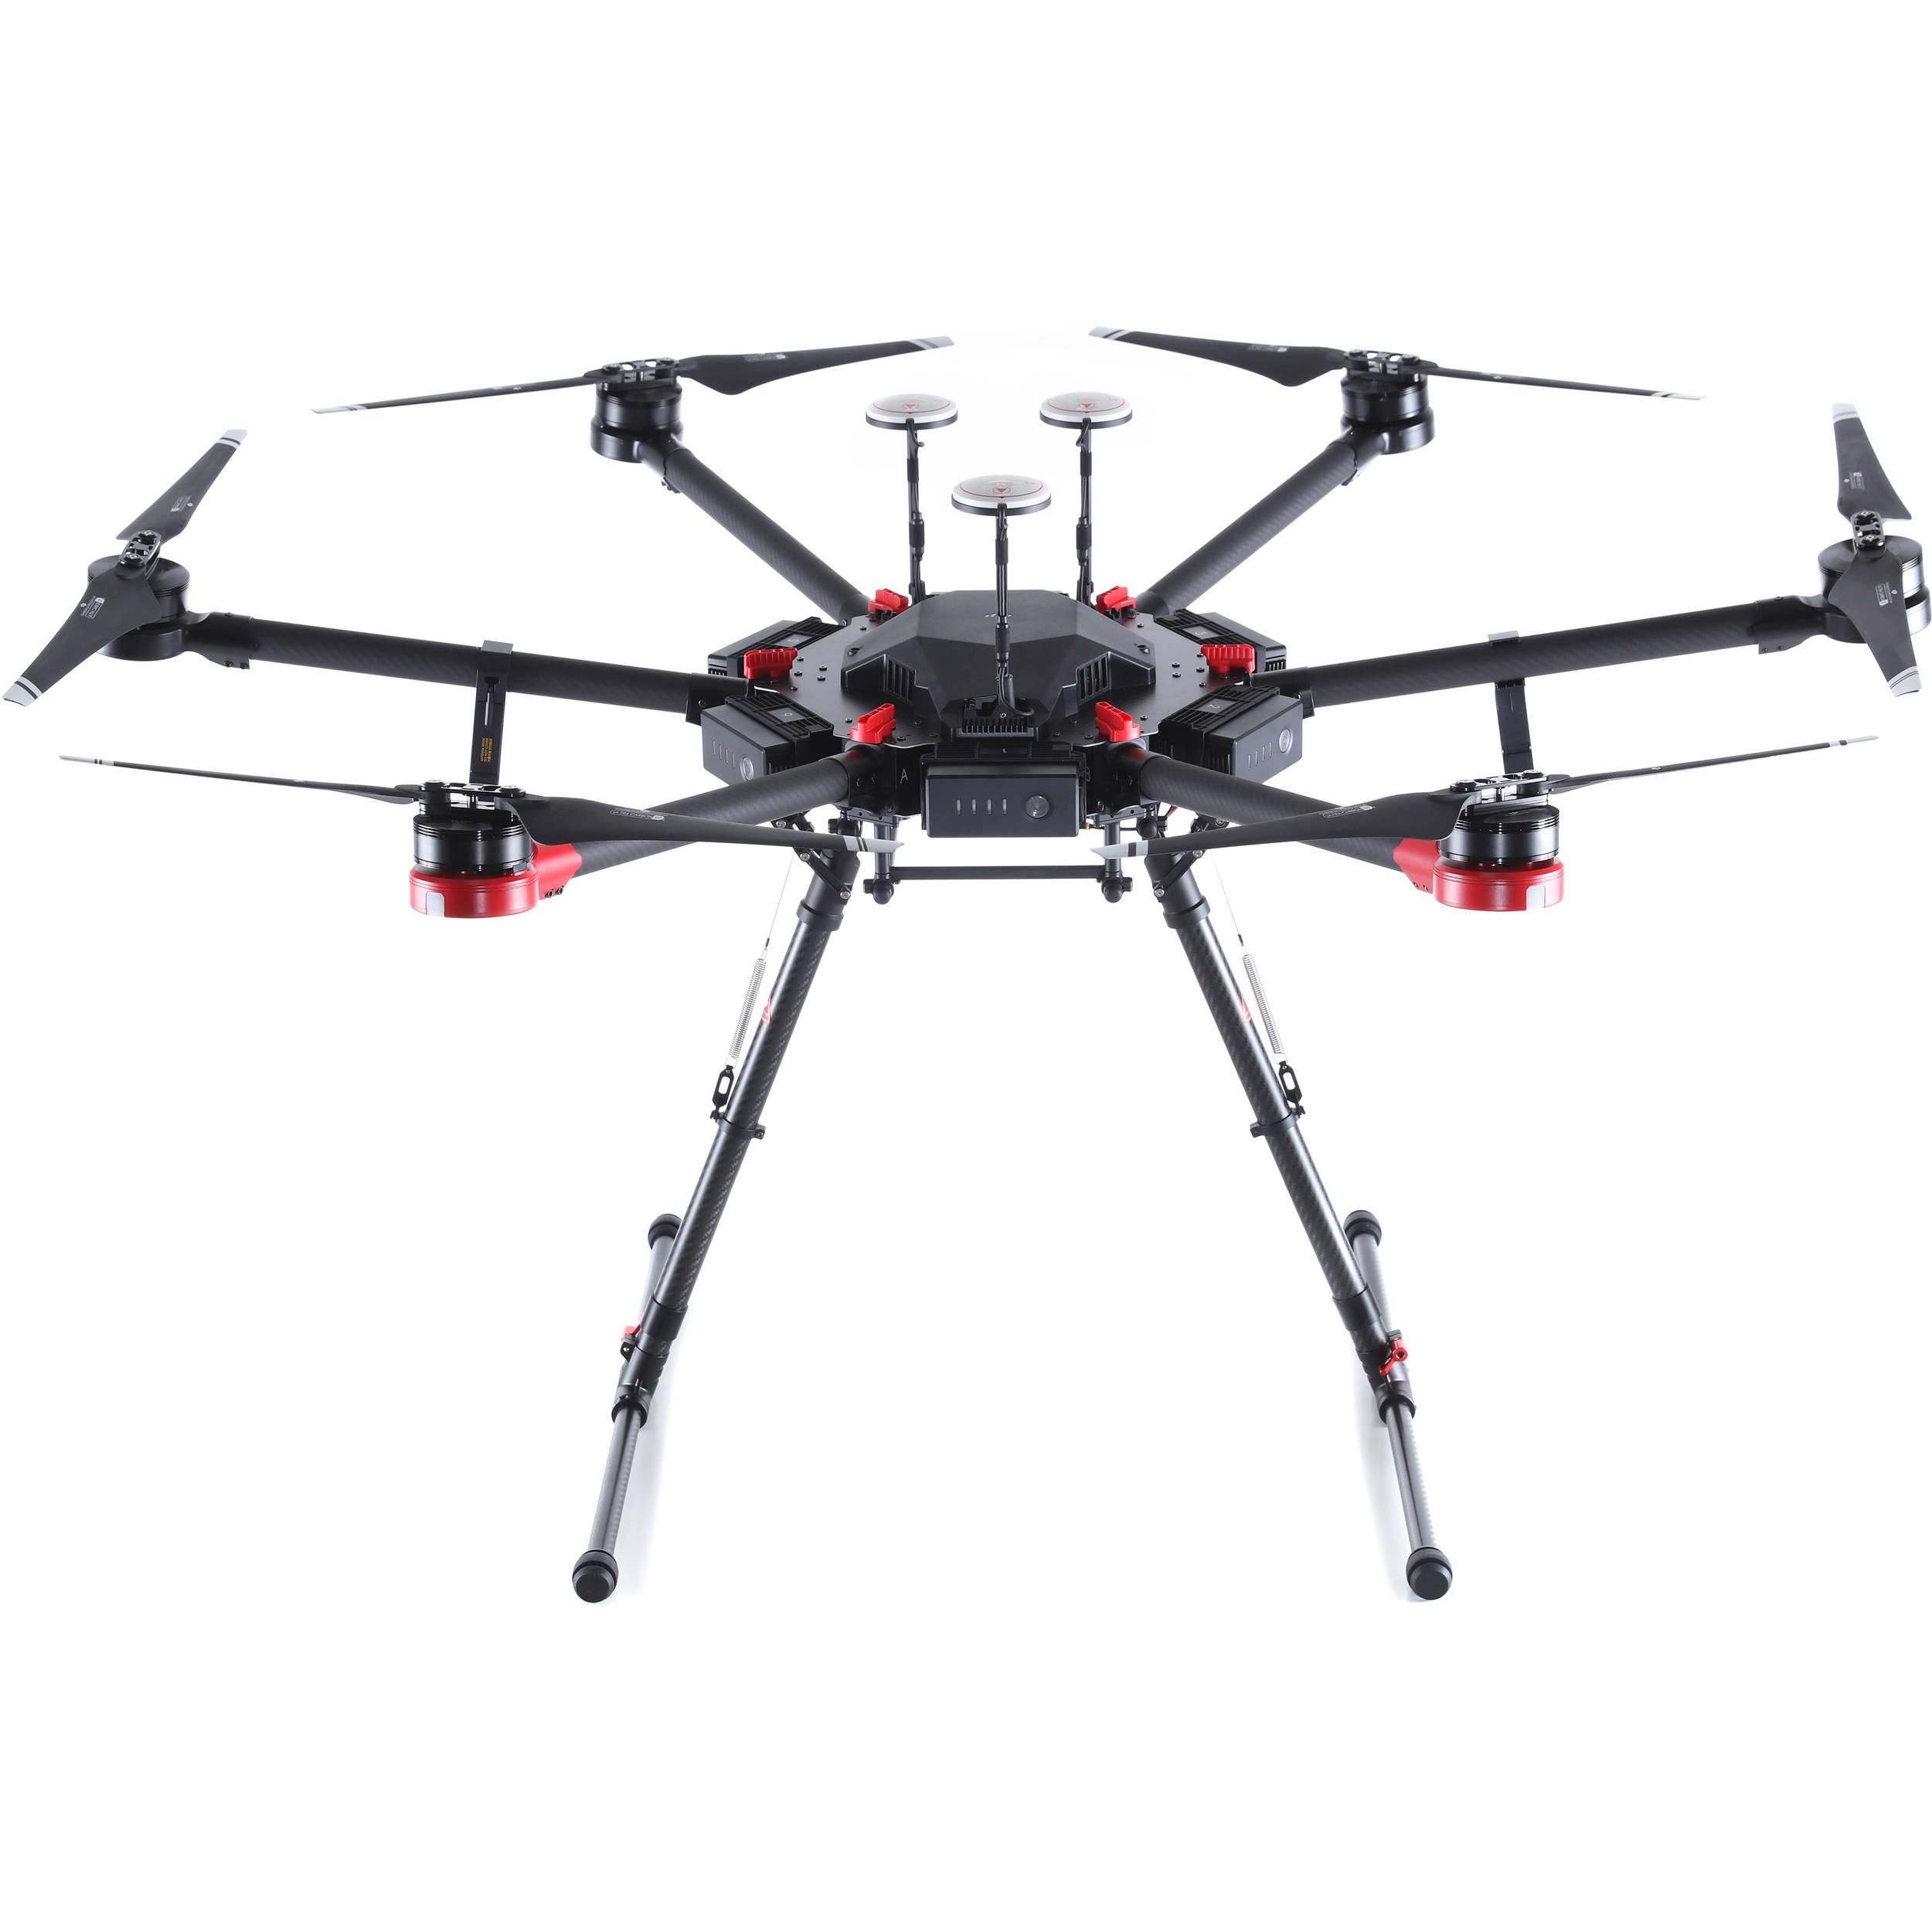
\includegraphics[width=0.9\columnwidth]{Figures/M600.jpg}
    \caption{DJI Matrice 600 Pro}
    \label{fig:2}
\end{figure}

% REFERENCES FORMAT
% References must be the same font size as other body text.
\bibliographystyle{SIGCHI-Reference-Format}
\bibliography{ref}

\end{document}

